\documentclass[a4paper,11pt]{article}
\usepackage[utf8]{inputenc}
\usepackage[T1]{fontenc}
\usepackage{lmodern}

% Géométrie de page
\usepackage[top=2.2cm, bottom=2.2cm, left=2.2cm, right=2.2cm]{geometry}
\usepackage{setspace}
\setstretch{1.10}
\usepackage[skip=0.5em plus 0.1em]{parskip}

% Mathématiques
\usepackage{amsmath, amssymb, amsfonts, mathrsfs, bm}

% Tableaux et graphiques
\usepackage{booktabs, multirow, tabularx, array, makecell, colortbl}
\usepackage{xcolor}
\definecolor{primary}{RGB}{20, 50, 110}
\definecolor{secondary}{RGB}{0, 110, 180}
\definecolor{lightgray}{RGB}{245, 247, 250}
\definecolor{darkgray}{RGB}{60, 65, 75}
\definecolor{accentred}{RGB}{180, 30, 30}

% TikZ et Pgfplots
\usepackage{tikz}
\usepackage{pgfplots}
\pgfplotsset{compat=1.18}
\usetikzlibrary{calc,positioning,shapes.geometric,arrows.meta}

% Flottants et figures
\usepackage{graphicx}
\usepackage{float}
\usepackage{caption}
\captionsetup{font=small, labelfont={bf, color=primary}, skip=4pt}
\usepackage{subcaption}

% En-têtes et pieds de page
\usepackage{fancyhdr}
\pagestyle{fancy}
\fancyhf{}
\fancyhead[L]{\small\color{darkgray}\textit{M2 IAFA : Planification satellite SPOT-5}}
\fancyhead[R]{}
\fancyfoot[C]{\thepage}
\renewcommand{\headrulewidth}{0.4pt}
\renewcommand{\footrulewidth}{0.4pt}

% Liens
\usepackage{hyperref}
\hypersetup{
    colorlinks=true,
    linkcolor=primary,
    urlcolor=secondary,
    citecolor=primary
}

\newcommand{\R}{\mathbb{R}}
\newcommand{\N}{\mathbb{N}}
\newcommand{\B}{\{0, 1\}}

\begin{document}

% -------------------------------------------------------------
% En-tête du rapport
% -------------------------------------------------------------
\begin{center}
    {\large\scshape Université Paul Sabatier, Master 2 IAFA (IA \& Décision)}\\[0.2cm]
    {\normalsize Module d'Optimisation et Aide à la Décision}\\[0.5cm]
    
    \rule{\linewidth}{0.8pt}\\[0.3cm]
    {\LARGE\bfseries\color{primary} Planification des prises de vue du satellite SPOT-5}\\[0.15cm]
    {\large Modélisation en PLNE, prise en compte des incertitudes et résolution avec SCIP}\\[0.2cm]
    \rule{\linewidth}{0.8pt}\\[0.4cm]
    
    \begin{minipage}{0.60\textwidth}
        \begin{flushleft}
            \textbf{Étudiants :} Alex \textsc{Tsan}, Paul \textsc{Serratos}, Hadrien \textsc{Lagier}
        \end{flushleft}
    \end{minipage}
    \begin{minipage}{0.36\textwidth}
        \begin{flushright}
            \textbf{Enseignante :} Nahla \textsc{Ben Amor}
        \end{flushright}
    \end{minipage}
\end{center}

\renewcommand{\abstractname}{\large\bfseries\color{primary} Résumé}

\begin{abstract}
    Ce travail porte sur la modélisation et la résolution du problème d'ordonnancement des prises de vue pour un satellite d'observation terrestre (type SPOT-5). Le problème consiste à sélectionner un ensemble d'images (mono ou stéréo) et à les affecter aux trois instruments embarqués afin de maximiser le gain espéré, tout en respectant la capacité mémoire du satellite, les contraintes de non-chevauchement temporel et les temps de dépointage des miroirs. Nous intégrons les incertitudes sur la couverture nuageuse et sur les pannes d'instruments directement dans l'espérance de gain de la fonction objectif. Le modèle est formulé en Programmation Linéaire en Nombres Entiers (PLNE) et résolu avec le solveur SCIP via \texttt{PySCIPOpt}. Nous présentons ensuite la validation sur des petites instances, puis l'analyse détaillée des plans obtenus sur les instances \texttt{spotProba4} et \texttt{spotProba5}, en étudiant notamment la réaction du modèle face à une défaillance instrumentale et aux variations météorologiques.
\end{abstract}

\vspace{0.3cm}
\hrule
\vspace{0.4cm}

% -------------------------------------------------------------
% Sections du rapport
% -------------------------------------------------------------
\section{Introduction et Contexte du Problème}

Le sujet porte sur la planification des prises de vue du satellite d'observation optique SPOT-5. Ce problème consiste à décider, pour chaque journée, quelles images seront acquises le lendemain et par quel instrument, à partir d'un ensemble de commandes de clients du monde entier.

\subsection{Caractéristiques Orbitales et Instruments}
D'après les spécifications fournies :
\begin{itemize}
    \item Orbite : circulaire (altitude constante de l'ordre de $700\text{ km}$), quasi-polaire et héliosynchrone, décrivant environ 14 révolutions de $100\text{ minutes}$ par jour avec un cycle de 25 jours. Les prises de vue optiques sont réalisées exclusivement de jour, lors de la descente du pôle Nord vers le pôle Sud.
    \item Instruments d'observation : le satellite embarque trois instruments optiques identiques équipés chacun d'un miroir de visée indépendant orientable latéralement, couvrant un corridor au sol de $800\text{ km}$ de large ($400\text{ km}$ de chaque côté de la trace) :
    \begin{itemize}
        \item Instrument 1 (Avant) : pointeur incliné vers l'avant dans le plan orbital (angle fixe d'environ $+25^\circ$).
        \item Instrument 2 (Nadir / Centre) : pointeur vertical vers le centre de la Terre ($0^\circ$).
        \item Instrument 3 (Arrière) : pointeur incliné vers l'arrière dans le plan orbital (angle fixe d'environ $-25^\circ$).
    \end{itemize}
    \item Images cibles : chaque commande correspond à une zone carrée d'environ $60\text{ km}$ de côté.
\end{itemize}

\begin{figure}[H]
    \centering
    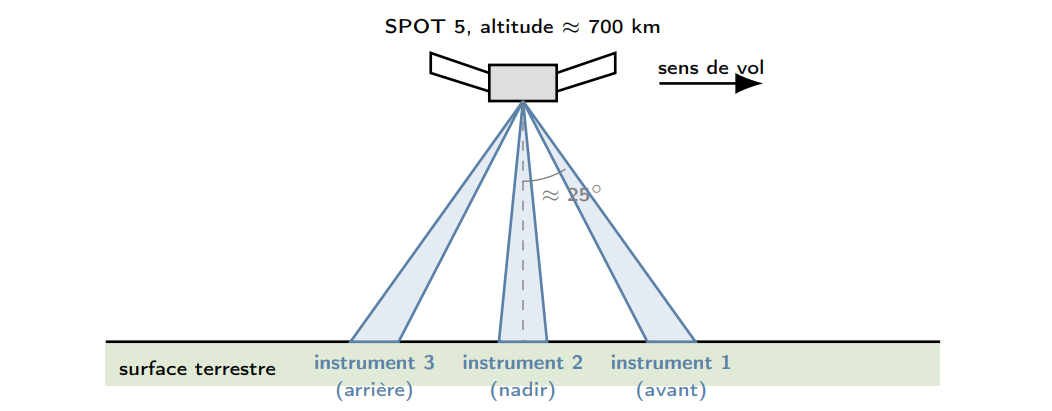
\includegraphics[width=0.78\textwidth]{spot_geometry.png}
    \caption{Disposition des trois instruments optiques de SPOT-5 le long de l'orbite (source : support de cours version slides).}
    \label{fig:spot_schema}
\end{figure}

\subsection{Types de Prises de Vue et Contraintes du Sujet}
Deux types de demandes coexistent :
\begin{itemize}
    \item Images monoscopiques ($TY=1$) : Une seule acquisition, réalisable par n'importe lequel des trois instruments.
    \item Images stéréoscopiques ($TY=2$) : Deux images acquises au cours de la même révolution pour restituer le relief, requérant obligatoirement les instruments 1 (avant) et 3 (arrière), sans utiliser l'instrument 2.
\end{itemize}

La planification doit respecter les contraintes physiques et technologiques définies dans l'énoncé :
\begin{itemize}
    \item Capacité mémoire : La quantité totale de mémoire $PM$ stockée à bord ne doit pas dépasser la capacité maximale $PM_{\max}$ du satellite (la mémoire requise est déjà doublée pour les stéréos dans les données).
    \item Non-chevauchement temporel et dépointage : Deux images programmées sur un même instrument ne peuvent pas se chevaucher et doivent laisser un délai suffisant pour la rotation angulaire du miroir à la vitesse $V_I$.
    \item Incertitudes : Les images nuageuses ne sont pas vendues (intervalle de probabilité de nuages $[ProbaInf, ProbaSup]$). De plus, chaque instrument présente une probabilité de défaillance ($Failure$).
\end{itemize}

\section{Modélisation Mathématique (PLNE)}

Nous formulons le problème sous forme d'un programme linéaire en nombres entiers. Cette section présente les ensembles, paramètres, variables de décision et contraintes en notation mathématique.

\subsection{Ensembles et Paramètres}
\begin{itemize}
    \item $\mathcal{I} = \{0, \dots, N-1\}$ : ensemble des demandes d'images, partitionné en $\mathcal{I}_{\text{mono}} = \{i \in \mathcal{I} \mid TY_i = 1\}$ et $\mathcal{I}_{\text{stereo}} = \{i \in \mathcal{I} \mid TY_i = 2\}$.
    \item $\mathcal{J} = \{0, 1, 2\}$ : ensemble des trois instruments (0 pour l'instrument 1 avant, 1 pour l'instrument 2 nadir, 2 pour l'instrument 3 arrière).
\end{itemize}

Pour chaque image $i \in \mathcal{I}$ et instrument $j \in \mathcal{J}$, les paramètres sont :
\begin{itemize}
    \item $PA_i \in \R_+$ : gain financier rapporté par l'image $i$ si elle est réussie.
    \item $PM_i \in \N^*$ : mémoire requise par l'image $i$ (déjà doublée pour les stéréos dans les données).
    \item $PM_{\max} \in \N^*$ : capacité mémoire totale disponible à bord.
    \item $DU \in \N^*$ : durée d'une prise de vue (identique pour toutes les images, en secondes).
    \item $V_I \in \R_+^*$ : vitesse de rotation du miroir de visée (en degrés par seconde).
    \item $DD_{i,j} \in \N$ : date de début de l'acquisition de l'image $i$ par l'instrument $j$ (en secondes).
    \item $AN_{i,j} \in \R$ : angle de dépointage nécessaire pour pointer la cible $i$ avec l'instrument $j$.
\end{itemize}

\subsection{Variables de Décision}
Nous définissons deux jeux de variables binaires :
\begin{itemize}
    \item $x_i \in \{0, 1\}$ pour tout $i \in \mathcal{I}$ : vaut 1 si l'image $i$ est sélectionnée dans le plan, 0 sinon.
    \item $y_{i,j} \in \{0, 1\}$ pour tout $i \in \mathcal{I}, j \in \mathcal{J}$ : vaut 1 si l'image $i$ est affectée à l'instrument $j$, 0 sinon.
\end{itemize}

\subsection{Contraintes de Faisabilité}

\subsubsection{1. Affectation des Images Mono et Stéréo}
Une image mono sélectionnée doit être affectée à exactement un instrument :
\begin{equation}
    \sum_{j \in \mathcal{J}} y_{i,j} = x_i \quad \forall i \in \mathcal{I}_{\text{mono}} \label{eq:mono}
\end{equation}

Une image stéréo sélectionnée exige obligatoirement les instruments 0 et 2, et interdit l'instrument 1 :
\begin{align}
    y_{i,0} &= x_i \quad \forall i \in \mathcal{I}_{\text{stereo}} \label{eq:stereo0} \\
    y_{i,1} &= 0 \quad \forall i \in \mathcal{I}_{\text{stereo}} \label{eq:stereo1} \\
    y_{i,2} &= x_i \quad \forall i \in \mathcal{I}_{\text{stereo}} \label{eq:stereo2}
\end{align}

\subsubsection{2. Capacité Mémoire}
La somme des tailles des images retenues ne doit pas dépasser la mémoire embarquée :
\begin{equation}
    \sum_{i \in \mathcal{I}} PM_i \cdot x_i \leq PM_{\max} \label{eq:mem}
\end{equation}

\subsubsection{3. Non-Chevauchement et Rotation du Miroir}
Considérons deux images $i_1 < i_2$ candidates sur un même instrument $j$. Le temps entre leurs débuts doit être suffisant pour réaliser la première prise ($DU$) et faire pivoter le miroir de l'angle $AN_{i_1,j}$ à l'angle $AN_{i_2,j}$ à la vitesse $V_I$ :
\begin{equation}
    \Delta t = |DD_{i_1,j} - DD_{i_2,j}| \geq DU + \frac{|AN_{i_1,j} - AN_{i_2,j}|}{V_I}
\end{equation}
Sous forme linéaire (sans division), deux images $i_1, i_2$ sont en conflit cinématique sur l'instrument $j$ dès que :
\begin{equation}
    |DD_{i_1,j} - DD_{i_2,j}| \cdot V_I < DU \cdot V_I + |AN_{i_1,j} - AN_{i_2,j}| \label{eq:conflit_cond}
\end{equation}
Pour chaque paire en conflit sur l'instrument $j$, au plus une des deux peut être allouée à cet instrument :
\begin{equation}
    y_{i_1,j} + y_{i_2,j} \leq 1 \label{eq:disjonction}
\end{equation}

\noindent\textit{Remarque sur les valeurs fictives et l'exclusivité :}
Pour les images stéréo, la date $DD[i][1]=0$ et l'angle $AN[i][1]=0$ sont de simples valeurs de remplissage dans les données (puisque la stéréo n'utilise jamais le nadir). Ces valeurs fictives sont donc ignorées lors de la génération des conflits cinématiques sur l'instrument 1 pour éviter toute contrainte artificielle. Par ailleurs, la contrainte d'exclusivité (un instrument ne peut réaliser deux acquisitions simultanées) est naturellement couverte par l'inéquation~(\ref{eq:disjonction}), car deux acquisitions simultanées se chevauchent obligatoirement.

\section{Traitement de l'Incertitude}

Deux facteurs aléatoires conditionnent la réussite d'une prise de vue : la météo au-dessus de la cible et la fiabilité des instruments du satellite.

\subsection{Description des Incertitudes}
\begin{itemize}
    \item Couverture nuageuse : Une image couverte de nuages est inexploitable et n'est pas vendue. Les prévisions fournissent un intervalle de probabilité de présence de nuages $p_i^{\text{cloud}} \in [p_i^{\inf}, p_i^{\sup}]$. La probabilité d'avoir un ciel clair $p_i^{\text{clear}} = 1 - p_i^{\text{cloud}}$ appartient donc à l'intervalle $[1 - p_i^{\sup}, 1 - p_i^{\inf}]$.
    \item Pannes matérielles : Chaque instrument $j \in \mathcal{J}$ présente une probabilité de panne $f_j \in [0, 1]$. La probabilité qu'il fonctionne correctement est donc $1 - f_j$.
\end{itemize}

\subsection{Hypothèses de décomposition de l'utilité espérée}
Pour décomposer l'espérance de gain globale de manière additive image par image dans la fonction objectif, trois hypothèses fondamentales sont requises :
\begin{itemize}
    \item Indépendance météo / instrument : La nébulosité au sol et l'état matériel d'un instrument sont des événements indépendants.
    \item Indépendance des pannes entre instruments : Les défaillances des instruments 0 et 2 sont statistiquement indépendantes, de sorte que la probabilité conjointe de bon fonctionnement pour une image stéréo est $(1 - f_0)(1 - f_2)$.
    \item Linéarité de l'utilité financière : La valeur globale d'un ensemble d'images réussies est égale à la somme de leurs gains respectifs $PA_i$.
\end{itemize}

\subsection{Critères de décision pour la Météo}
Face à l'intervalle $[p_i^{\inf}, p_i^{\sup}]$, plusieurs critères peuvent être appliqués pour fixer $p_i^{\text{clear}}$ :
\begin{itemize}
    \item Pessimiste (Wald / Maximin) : On retient la pire météo possible, soit $p_i^{\text{clear}} = 1 - p_i^{\sup}$.
    \item Moyen (Laplace) : En l'absence de loi de probabilité \textit{a priori}, on prend la moyenne : $p_i^{\text{clear}} = 1 - \frac{p_i^{\inf} + p_i^{\sup}}{2}$.
    \item Optimiste (Maximax) : On retient le meilleur cas possible : $p_i^{\text{clear}} = 1 - p_i^{\inf}$.
\end{itemize}

\subsection{Calcul de l'espérance de gain et fonction objectif}
Sous ces hypothèses, l'espérance de gain s'exprime de façon unitaire :
\begin{itemize}
    \item Pour une image mono ($TY_i = 1$) allouée à l'instrument $j$ :
    \begin{equation}
        \mathbb{E}[\text{Gain}_i \mid y_{i,j}=1] = PA_i \cdot p_i^{\text{clear}} \cdot (1 - f_j)
    \end{equation}
    \item Pour une image stéréo ($TY_i = 2$) sélectionnée ($x_i=1$) :
    \begin{equation}
        \mathbb{E}[\text{Gain}_i \mid x_i=1] = PA_i \cdot p_i^{\text{clear}} \cdot (1 - f_0) \cdot (1 - f_2)
    \end{equation}
\end{itemize}

La fonction objectif globale maximisée par SCIP s'écrit alors :
\begin{equation}
    \max \quad \mathbb{E}[\mathcal{Z}] = \sum_{i \in \mathcal{I}_{\text{mono}}} \sum_{j \in \mathcal{J}} \left[ PA_i \cdot p_i^{\text{clear}} \cdot (1 - f_j) \right] y_{i,j} \;+\; \sum_{i \in \mathcal{I}_{\text{stereo}}} \left[ PA_i \cdot p_i^{\text{clear}} \cdot (1 - f_0)(1 - f_2) \right] x_i \label{eq:obj}
\end{equation}

\subsection{Justification du Critère Retenu}
Pour la planification nominale, nous retenons l'espérance de gain sous critère pessimiste. La mémoire à bord étant une ressource dure et non renouvelable, planifier une image très incertaine prive d'autres cibles sûres de pouvoir être acquises. Le critère pessimiste garantit un plan robuste et prévisible.

\section{Implémentation et Utilisation de l'IA}

\subsection{Architecture Logicielle}
Le projet est développé en Python avec le solveur de programmation mathématique SCIP via la bibliothèque \texttt{PySCIPOpt}. Le code est structuré en deux modules principaux :
\begin{itemize}
    \item \texttt{spot\_solver.py} : Contient la classe \texttt{SpotInstance} pour charger les données et détecter les conflits cinématiques, ainsi que la fonction \texttt{solve\_spot} qui instancie les variables, pose les contraintes et résout le modèle avec SCIP.
    \item \texttt{app.py} : Une interface web développée avec Streamlit et Plotly permettant de visualiser le diagramme de Gantt des acquisitions, d'inspecter les conflits, de comparer les scénarios météo et d'exporter les plannings en CSV/JSON.
    \item \texttt{benchmark\_report.py} : Un script d'automatisation exécutant l'ensemble des scénarios et variations paramétriques pour collecter les indicateurs d'optimisation.
\end{itemize}

\subsection{Extrait de code de la modélisation}
L'extrait suivant illustre la construction de la fonction objectif avec prise en compte des probabilités dans le code :

\begin{verbatim}
# Calcul des termes de l'espérance de gain
obj_terms = []
for i in range(nb_images):
    if instance.TY[i] == 1:
        # Mono : dépend de l'instrument choisi et de son taux de panne
        for j in range(nb_instruments):
            coef = instance.PA[i] * p_clear[i] * (1.0 - failure[j])
            obj_terms.append(coef * assigned_to[i][j])
    else:
        # Stéréo : requiert simultanément les instruments 0 et 2
        f0, f2 = failure[0], failure[2]
        coef = instance.PA[i] * p_clear[i] * (1.0 - f0) * (1.0 - f2)
        obj_terms.append(coef * selection[i])

model.setObjective(quicksum(obj_terms), sense="maximize")
\end{verbatim}

\subsection{Mention de l'Usage de l'IA}
Conformément aux consignes du cours :
\begin{itemize}
    \item Ce qui a été fait avec l'IA : Nous avons utilisé un assistant IA pour accélérer le développement de l'interface graphique Streamlit (notamment la mise en forme du graphique de Gantt sous Plotly), pour réaliser le script de benchmark automatisé (\texttt{benchmark\_report.py}) et pour générer la structure du fichier de mise en page \LaTeX.
    \item Ce qui n'a pas été fait avec l'IA : La formulation du modèle mathématique (variables de décision, contraintes de cohérence stéréo, disjonctions cinématiques, formalisation de l'espérance), le choix des critères sous incertitude ainsi que l'analyse critique des résultats et des arbitrages ont été réalisés directement par nos soins.
\end{itemize}

\section{Validation du Modèle sur Petites Instances}

Pour vérifier nos contraintes et notre fonction objectif, nous avons testé le modèle sur les trois petites instances de test fournies (\texttt{spotProba1}, \texttt{spotProba2}, \texttt{spotProba3}).

\subsection{Description des Cas de Test}
\begin{itemize}
    \item \texttt{spotProba1} : Configuration nominale ($PM_{\max} = 50$, $DU = 20\text{ s}$). Les 3 images tiennent en mémoire ($10 + 20 + 10 = 40 \leq 50$) et leurs créneaux temporels ne sont pas en conflit. Le gain optimal attendu est de 70.0.
    \item \texttt{spotProba2} : La capacité mémoire est réduite à $PM_{\max} = 35$. Il devient impossible de garder les 3 images (coût 40). Le solveur doit choisir les images 1 et 2 (gain $20 + 40 = 60.0$, mémoire 30).
    \item \texttt{spotProba3} : La durée d'acquisition passe à $DU = 100\text{ s}$. Un conflit temporel apparaît entre l'image 0 et les autres sur les instruments, forçant à écarter l'image 0. Le gain optimal est de 60.0.
\end{itemize}

\subsection{Résultats Obtenus}
Le tableau~\ref{tab:validation} résume les résultats obtenus par SCIP. Les valeurs optimales et les sélections d'images correspondent exactement aux attendus de l'énoncé.

\begin{table}[H]
\centering
\small
\begin{tabularx}{\textwidth}{lcccccX}
\toprule
\textbf{Instance} & \textbf{$PM_{\max}$} & \textbf{$DU$ (s)} & \textbf{Statut} & \textbf{Gain $\mathbb{E}[\mathcal{Z}]$} & \textbf{Mémoire} & \textbf{Images Retenues} \\
\midrule
\texttt{spotProba1} & 50 & 20 & Optimal & 70.0 & 40 / 50 & $\{0, 1, 2\}$ \\
\texttt{spotProba2} & 35 & 20 & Optimal & 60.0 & 30 / 35 & $\{1, 2\}$ \\
\texttt{spotProba3} & 50 & 100 & Optimal & 60.0 & 30 / 50 & $\{1, 2\}$ \\
\bottomrule
\end{tabularx}
\caption{Validation sur les trois instances de test de base (sans incertitude).}
\label{tab:validation}
\end{table}

\subsection{Tests avec Incertitude sur \texttt{spotProba1}}
Nous avons également testé les variantes stochastiques commentées dans \texttt{spotProba1.py} :
\begin{itemize}
    \item Nuages avec $p=0.10$ constant : Le gain optimal obtenu est $70 \times 0.9 = 63.00$ (valeur attendue : 63).
    \item Nuages dans $[0.10, 0.30]$ (Pessimiste) : Le gain obtenu est $70 \times 0.7 = 49.00$ (valeur attendue : 49).
    \item Panne de l'instrument 2 ($Failure=[0, 1, 0]$) : L'instrument nadir étant indisponible, l'image stéréo 1 (instruments 1 et 3) et l'image mono 2 sont sélectionnées. Le gain est de 60.00.
    \item Incertitudes mixtes sévères : Avec $p^{\sup} = [0.1, 0.5, 0.9]$ et $Failure = [0.01, 0.9, 0.01]$, le modèle donne une espérance de 14.661, ce qui correspond exactement à la valeur théorique mentionnée dans le sujet.
\end{itemize}

Ces tests confirment que la modélisation des contraintes et du calcul d'espérance est correcte.

\section{Résultats et Analyse sur \texttt{spotProba4}}

L'instance \texttt{spotProba4} comporte 20 demandes d'images (14 mono et 6 stéréo), avec $PM_{\max} = 150$, $DU = 20\text{ s}$ et $V_I = 1^\circ/\text{s}$. Les instruments sont fiables ($Failure = [0, 0, 0]$), mais la météo est contrastée : $p^{\sup} = 0.10$ pour les monos (météo favorable) et $p^{\sup} = 0.70$ pour les stéréos (fort risque de nuages).

\subsection{Comparaison des Politiques Météo : Écart de Valeur et de Sélection}
Le tableau~\ref{tab:spot4_comparaison} compare les résultats obtenus selon l'hypothèse météo retenue.

\begin{table}[H]
\centering
\small
\begin{tabularx}{\textwidth}{lXXXXc}
\toprule
\textbf{Scénario Météo} & \textbf{Gain $\mathbb{E}[\mathcal{Z}]$} & \textbf{Sélection} & \textbf{Mono / Stéréo} & \textbf{Mémoire} & \textbf{Temps SCIP (ms)} \\
\midrule
Pessimiste (Wald) & 333.00 & 14 / 20 & 14 M / 0 S & 140 / 150 & 22.4 \\
Moyen (Laplace) & 362.00 & 13 / 20 & 11 M / 2 S & 150 / 150 & 7.6 \\
Optimiste (Maximax) & 400.00 & 13 / 20 & 11 M / 2 S & 150 / 150 & 6.3 \\
Déterministe (sans nuages) & 400.00 & 13 / 20 & 11 M / 2 S & 150 / 150 & 19.8 \\
\bottomrule
\end{tabularx}
\caption{Comparaison des plans obtenus sur \texttt{spotProba4} selon le critère météo.}
\label{tab:spot4_comparaison}
\end{table}

\noindent\textit{Écart entre plan pessimiste et plan optimiste :} Les deux plans ne diffèrent pas seulement par leur valeur objective ($333.00$ contre $400.00$), mais également par la nature des images sélectionnées :
\begin{itemize}
    \item Plan pessimiste : 14 images retenues (14 mono et 0 stéréo), mémoire $140 / 150$. Les images sélectionnées sont $\{0, 2, 4, 5, 6, 8, 9, 10, 12, 14, 15, 16, 18, 19\}$.
    \item Plan optimiste : 13 images retenues (11 mono et 2 stéréo), mémoire saturée à $150 / 150$. Les images mono 4, 10 et 15 sont éliminées pour faire place aux 2 stéréos 3 et 13.
\end{itemize}

\subsection{Détail du Plan Optimal (Scénario Pessimiste)}
Le tableau~\ref{tab:spot4_schedule} présente l'ordonnancement exact des 14 prises de vue dans le plan pessimiste.

\begin{table}[H]
\centering
\small
\begin{tabularx}{\textwidth}{ccXcccc}
\toprule
\textbf{ID} & \textbf{Type} & \textbf{Instrument Alloué} & \textbf{Début (s)} & \textbf{Fin (s)} & \textbf{Gain Facial} & \textbf{$P(\text{Ciel Clair})$} \\
\midrule
0 & Mono & Instrument 2 (Nadir) & 200 & 220 & 10.0 & 0.90 \\
5 & Mono & Instrument 1 (Avant) & 230 & 250 & 20.0 & 0.90 \\
2 & Mono & Instrument 2 (Nadir) & 250 & 270 & 40.0 & 0.90 \\
8 & Mono & Instrument 1 (Avant) & 290 & 310 & 50.0 & 0.90 \\
4 & Mono & Instrument 2 (Nadir) & 320 & 340 & 10.0 & 0.90 \\
12 & Mono & Instrument 1 (Avant) & 330 & 350 & 50.0 & 0.90 \\
6 & Mono & Instrument 2 (Nadir) & 350 & 370 & 40.0 & 0.90 \\
9 & Mono & Instrument 2 (Nadir) & 400 & 420 & 20.0 & 0.90 \\
14 & Mono & Instrument 1 (Avant) & 420 & 440 & 20.0 & 0.90 \\
16 & Mono & Instrument 1 (Avant) & 450 & 470 & 40.0 & 0.90 \\
19 & Mono & Instrument 1 (Avant) & 500 & 520 & 20.0 & 0.90 \\
10 & Mono & Instrument 3 (Arrière) & 500 & 520 & 10.0 & 0.90 \\
15 & Mono & Instrument 2 (Nadir) & 530 & 550 & 10.0 & 0.90 \\
18 & Mono & Instrument 2 (Nadir) & 570 & 590 & 30.0 & 0.90 \\
\bottomrule
\end{tabularx}
\caption{Planning détaillé des prises de vue sur \texttt{spotProba4} (Politique Pessimiste).}
\label{tab:spot4_schedule}
\end{table}

\subsection{Analyse causale des images écartées}
Sur les 20 images candidates de \texttt{spotProba4}, certaines sont écartées pour des motifs précis :
\begin{itemize}
    \item Écartées pour cause de risque nuageux excessif (stéréos 3 et 13 en pessimiste) : Avec $p^{\sup}=0.70$, leur probabilité de ciel clair est de $0.30$. Une stéréo à gain facial 30 ne rapporte en espérance que $30 \times 0.30 = 9.0$ pour un coût mémoire de 20. Deux monos à gain 50 (images 8 et 12) rapportent $2 \times (50 \times 0.90) = 90.0$, soit dix fois plus. Le solveur écarte donc les stéréos en pessimiste.
    \item Écartées pour cause de mémoire (monos 4, 10, 15 en optimiste) : Lorsque la météo devient favorable, le solveur préfère allouer les 40 unités de mémoire aux stéréos 3 et 13, ce qui oblige à écarter ces trois petites monos à gain facial modeste ($PA=10$).
    \item Écartées systématiquement dans tous les scénarios (stéréos 1, 7, 11, 17) : Ces quatre stéréos ont un gain facial trop faible ($PA=10$ ou $20$) par rapport à leur coût mémoire ($PM=20$) et aux conflits temporels qu'elles engendrent simultanément sur les instruments 1 et 3.
\end{itemize}

\section{Résultats et Analyse sur \texttt{spotProba5}}

L'instance \texttt{spotProba5} comporte 40 demandes d'images, une capacité mémoire $PM_{\max} = 300$, une nébulosité variable croissante le long de la trace ($p_i^{\sup} \in [0.1, 0.7]$), et une défaillance importante sur l'instrument 3 :
\begin{equation}
    Failure = [0.001, \, 0.001, \, 0.70]
\end{equation}

\subsection{Comparaison des Scénarios Météo sur \texttt{spotProba5}}
Le tableau~\ref{tab:spot5_comparaison} présente les résultats obtenus pour chaque hypothèse météorologique sous la panne nominale de l'instrument 3.

\begin{table}[H]
\centering
\small
\begin{tabularx}{\textwidth}{lXXXXc}
\toprule
\textbf{Scénario Météo} & \textbf{Gain $\mathbb{E}[\mathcal{Z}]$} & \textbf{Sélection} & \textbf{Mono / Stéréo} & \textbf{Mémoire} & \textbf{Temps SCIP (ms)} \\
\midrule
Pessimiste (Wald) & 553.65 & 27 / 40 & 24 M / 3 S & 300 / 300 & 14.4 \\
Moyen (Laplace) & 615.88 & 27 / 40 & 24 M / 3 S & 300 / 300 & 12.0 \\
Optimiste (Maximax) & 678.12 & 27 / 40 & 24 M / 3 S & 300 / 300 & 12.3 \\
Déterministe (sans nuages) & 789.22 & 28 / 40 & 26 M / 2 S & 300 / 300 & 10.6 \\
\bottomrule
\end{tabularx}
\caption{Performances sur l'instance \texttt{spotProba5} avec panne à 70\% sur l'instrument 3.}
\label{tab:spot5_comparaison}
\end{table}

\subsection{Déformation du plan par rapport à \texttt{spotProba4}}
L'instrument 3 étant peu fiable ($f_2=0.70$), toute image stéréo en dépend obligatoirement. Le tableau~\ref{tab:spot5_failure_impact} met en évidence la déformation structurelle du plan par rapport à une situation sans panne.

\begin{table}[H]
\centering
\small
\begin{tabularx}{\textwidth}{lXXXXc}
\toprule
\textbf{État de l'Instrument 3} & \textbf{Gain Espéré} & \textbf{Mono / Stéréo} & \textbf{Mémoire} & \textbf{Charge Inst. 1 / 2 / 3} \\
\midrule
Sans panne ($f_2 = 0$) & 621.00 & 20 M / 5 S & 300 / 300 & 12 / 10 / 8 \\
Panne partielle ($f_2 = 0.70$) & 553.65 & 24 M / 3 S & 300 / 300 & 15 / 12 / 3 \\
Panne totale ($f_2 = 1.00$) & 534.47 & 24 M / 0 S & 240 / 300 & 13 / 11 / 0 \\
\bottomrule
\end{tabularx}
\caption{Déformation du plan d'acquisition selon le niveau de panne de l'instrument 3 (\texttt{spotProba5}).}
\label{tab:spot5_failure_impact}
\end{table}

\noindent\textit{Analyse de la déformation :}
\begin{itemize}
    \item Report intégral des images mono sur les instruments 1 et 2 : L'instrument 3 ayant 70\% de risque d'échec, toute mono qui lui serait affectée verrait son gain divisé par plus de 3. Le solveur choisit donc d'affecter 0 image mono sur l'instrument 3. La totalité des 24 monos est absorbée par les instruments sains 1 (15 prises) et 2 (12 prises). Les 3 seules prises affectées à l'instrument 3 correspondent aux 3 stéréos obligées.
    \item Sélection ciblée des stéréos à très fort gain : Alors que dans \texttt{spotProba4} aucune stéréo n'était gardée en pessimiste à cause des nuages, dans \texttt{spotProba5} le solveur retient 3 stéréos (images 1, 11 et 20) car leur gain facial élevé ($PA=40$ pour l'image 20) compense le facteur $(1-f_0)(1-f_2) \approx 0.30$ et leurs créneaux temporels n'entrent pas en conflit avec les monos majeures.
\end{itemize}

\subsection{Analyse des Images Systématiquement Écartées}
Sur les 40 images candidates de \texttt{spotProba5}, 12 images sont systématiquement écartées quel que soit le scénario météo :
\begin{itemize}
    \item Écartées pour cause de risque cumulé (panne + nuage) : les images stéréo 3, 7, 13, 17, 21, 23, 27, 31, 33, 37 ont une espérance de gain trop faible pour justifier les 20 unités de mémoire et l'occupation de l'instrument 3 dégradé.
    \item Écartées pour cause de conflit cinématique direct : certaines images mono comme l'image 27 et l'image 31 sont en conflit de dépointage miroir direct avec des images mono beaucoup plus rentables (ex: image 24 à gain 60 et image 28 à gain 50) programmées sur les mêmes créneaux.
    \item Sous-utilisation mémoire en panne totale : en cas de panne totale ($f_2=1$), les instruments 1 et 2 ne peuvent cinématiquement réaliser que 24 images mono (mémoire $240 / 300$). Ce sont les conflits temporels entre images qui limitent le plan, et non la mémoire.
\end{itemize}

\section{Analyse de Robustesse et Étude de Sensibilité}
\label{sec:robustesse}

\subsection{Robustesse des choix d'acquisition}
Pour un opérateur au sol, il est utile de savoir quelles images sont rentables quelle que soit la météo, et lesquelles ne valent la peine que si les conditions sont parfaites. Nous distinguons :
\begin{itemize}
    \item Images robustes ($\mathcal{S}_{\text{rob}}$) : Sélectionnées dans tous les scénarios météo (Pessimiste, Moyen, Optimiste, Déterministe).
    \item Images conditionnelles ($\mathcal{S}_{\text{cond}}$) : Retenues seulement lorsque les prévisions de nébulosité sont favorables.
\end{itemize}

Le tableau~\ref{tab:robustesse} détaille cette répartition sur les deux instances principales.

\begin{table}[H]
\centering
\small
\begin{tabularx}{\textwidth}{lccl}
\toprule
\textbf{Instance} & \textbf{Robustes} & \textbf{Conditionnelles} & \textbf{Indices des Images} \\
\midrule
\multirow{2}{*}{\texttt{spotProba4}} & \multirow{2}{*}{11 / 20 (55\%)} & \multirow{2}{*}{5 / 20 (25\%)} & $\mathcal{S}_{\text{rob}} = \{0, 2, 5, 6, 8, 9, 12, 14, 16, 18, 19\}$ \\
 & & & $\mathcal{S}_{\text{cond}} = \{3, 4, 10, 13, 15\}$ \\
\midrule
\multirow{2}{*}{\texttt{spotProba5}} & \multirow{2}{*}{25 / 40 (62\%)} & \multirow{2}{*}{5 / 40 (12\%)} & $\mathcal{S}_{\text{rob}} = \{0, 2, 4, 5, 6, 8, 9, 12, 14, 15, 16, 18, 19, 20,$ \\
 & & & \quad\qquad $22, 24, 25, 26, 28, 29, 32, 34, 35, 36, 38\}$ \\
 & & & $\mathcal{S}_{\text{cond}} = \{1, 10, 11, 30, 39\}$ \\
\bottomrule
\end{tabularx}
\caption{Classification des requêtes d'images selon leur robustesse face à la météo.}
\label{tab:robustesse}
\end{table}

\subsection{Sensibilité à la Vitesse du Miroir \texorpdfstring{($V_I$)}{(VI)}}
La vitesse de rotation $V_I$ du miroir conditionne le nombre de conflits cinématiques entre deux prises consécutives. Le tableau~\ref{tab:sensi_vi} montre l'évolution des conflits et du gain sur \texttt{spotProba4} quand $V_I$ varie de $0.2^\circ/\text{s}$ à $5.0^\circ/\text{s}$.

\begin{table}[H]
\centering
\small
\begin{tabularx}{\textwidth}{cXXXX}
\toprule
\textbf{Vitesse $V_I$ ($^\circ/\text{s}$)} & \textbf{Nombre de Conflits} & \textbf{Gain $\mathbb{E}[\mathcal{Z}]$} & \textbf{Images Retenues} & \textbf{Mémoire Utilisée} \\
\midrule
0.2 & 158 conflits & 315.00 & 12 & 120 / 150 \\
0.5 & 93 conflits & 330.00 & 14 & 150 / 150 \\
1.0 (nominal) & 62 conflits & 333.00 & 14 & 140 / 150 \\
2.0 & 50 conflits & 333.00 & 14 & 140 / 150 \\
5.0 & 42 conflits & 333.00 & 14 & 150 / 150 \\
\bottomrule
\end{tabularx}
\caption{Impact de la vitesse de rotation miroir $V_I$ sur \texttt{spotProba4} (Pessimiste).}
\label{tab:sensi_vi}
\end{table}

Constat : En dessous de $1.0^\circ/\text{s}$, la rotation du miroir est trop lente et engendre de multiples incompatibilités (158 conflits à $0.2^\circ/\text{s}$, limitant le gain à 315.0). Au-delà de $1.0^\circ/\text{s}$, le gain ne progresse plus : la capacité mémoire devient la seule contrainte active.

\subsection{Sensibilité à la Capacité Mémoire \texorpdfstring{($PM_{\max}$)}{(PMmax)}}
Le tableau~\ref{tab:sensi_pm} illustre l'effet d'une variation de la mémoire embarquée sur \texttt{spotProba4}.

\begin{table}[H]
\centering
\small
\begin{tabularx}{\textwidth}{cXXXX}
\toprule
\textbf{Mémoire $PM_{\max}$} & \textbf{Gain $\mathbb{E}[\mathcal{Z}]$} & \textbf{Images Retenues} & \textbf{Mémoire Utilisée} & \textbf{Taux d'Occupation} \\
\midrule
50 & 198.00 & 5 & 50 & 100.0\% (Saturée) \\
100 & 297.00 & 10 & 100 & 100.0\% (Saturée) \\
150 (nominal) & 333.00 & 14 & 140 & 93.3\% \\
200 & 339.00 & 15 & 160 & 80.0\% \\
300 & 339.00 & 15 & 160 & 53.3\% \\
\bottomrule
\end{tabularx}
\caption{Impact de la capacité mémoire $PM_{\max}$ sur \texttt{spotProba4} (Pessimiste).}
\label{tab:sensi_pm}
\end{table}

Constat : Jusqu'à $PM_{\max}=150$, la mémoire limite directement le plan. Au-delà de $PM_{\max}=200$, le gain plafonne définitivement à 339.0 : toutes les images temporellement compatibles ont déjà été programmées.

\section{Conclusion et Limites du Modèle}

\subsection{Ce que le modèle permet de conclure}
L'approche par programmation linéaire en nombres entiers (PLNE) proposée s'avère bien adaptée au problème de planification d'acquisitions pour SPOT-5 :
\begin{itemize}
    \item Résolution exacte très rapide : Le solveur SCIP trouve l'optimum prouvé en moins de $25\text{ ms}$ sur l'instance à 20 images, et en $14\text{ ms}$ sur celle à 40 images. Ces temps de calcul sont tout à fait compatibles avec une utilisation opérationnelle quotidienne au centre de contrôle au sol.
    \item Arbitrages clairs sous incertitude : En formulant l'espérance de gain dans l'objectif, le modèle arbitre rationnellement entre le gain facial, la probabilité de nébulosité et la mémoire consommée. Il élimine de lui-même les images stéréo quand leur risque nuageux est trop élevé, et réaffecte spontanément la charge sur les instruments sains en cas de panne matérielle.
    \item Aide à la décision : L'analyse de robustesse permet à l'opérateur d'identifier les images à confirmer sans risque (robustes) et celles qui dépendent fortement de la fiabilité des prévisions météo.
\end{itemize}

\subsection{Ce que le modèle ne permet pas de conclure}
Certaines hypothèses du modèle constituent des limites pratiques qu'il convient de garder à l'esprit :
\begin{itemize}
    \item Planification statique hors-ligne : Le plan est calculé au sol avant la passe du satellite. Le modèle ne permet pas une replanification dynamique à bord en temps réel si une caméra de nébulosité embarquée détecte une zone dégagée imprévue.
    \item Indépendance spatiale des nuages : Nous supposons que les probabilités de nuages sont indépendantes d'une image à l'autre. En réalité, deux cibles voisines sont souvent couvertes par la même masse nuageuse. Une modélisation par scénarios météo corrélés permettrait d'affiner encore ce point.
    \item Passage à l'échelle pour de très grands problèmes : Sur un horizon pluri-journalier ou pour une constellation complète de satellites (plusieurs centaines ou milliers d'images), le nombre de contraintes disjonctives (\ref{eq:disjonction}) augmenterait de façon quadratique. Il deviendrait alors pertinent d'explorer des méthodes de décomposition (comme la décomposition de Benders) ou des heuristiques de recherche locale.
\end{itemize}


\end{document}
